\input{_preamble}
\fancyhead[L]{\sffamily\small\color{black!55}ДЗ №3 · MapReduce и DuckDB поверх RustFS}
\fancyhead[R]{\sffamily\small\color{black!55}Вариант 10 «Аналитик»}
% Выводы и код рендерятся через minted (Pygments): listings переставляет символы на стыке «-» и кириллицы
\tcbuselibrary{minted}
\tcbset{termmint/.style={enhanced, breakable, listing engine=minted, listing only,
  minted options={fontsize=\scriptsize, breaklines, breakanywhere},
  colback=termbg, coltext=termfg, colframe=termframe, colbacktitle=termtitle, coltitle=termtitlefg,
  fonttitle=\sffamily\footnotesize\bfseries, arc=2.2mm, boxrule=0.6pt, left=2.2mm, right=2.2mm, top=1.4mm, bottom=1.4mm,
  toptitle=1.2mm, bottomtitle=1.2mm, before skip=9pt, after skip=9pt}}
\renewcommand{\evidence}[2]{\tcbinputlisting{termmint, minted language=console, minted style=monokai,
  title={#2\hfill\termdots}, listing file={evidence/#1}}}
% строки таблиц подключаются примитивом TeX: LaTeX-овский \input ломает выравнивание перед \bottomrule
\makeatletter\newcommand{\tabin}[1]{\@@input tables/#1.tex }\makeatother
\newtcblisting{sqlbox}[1]{termmint, minted language=sql, minted style=monokai, title={#1\hfill\termdots}}
\newcommand{\shot}[3]{\IfFileExists{../screens/#1}{\begin{figure}[H]\centering\framedgraphic[width=#2]{../screens/#1}\caption{#3}\end{figure}}{}}

\begin{document}

\begin{tcolorbox}[enhanced, colback=accent, colframe=accentdark, coltext=white, arc=3mm, boxrule=0pt,
  left=7mm, right=7mm, top=6mm, bottom=5mm, after skip=10pt, shadow={1mm}{-1mm}{0mm}{black!20}]
{\sffamily\bfseries\huge MapReduce и DuckDB поверх RustFS}\\[2.2mm]
{\sffamily\large Вариант 10 «Аналитик»: навыки, пары и тройки навыков, влияние на зарплату, регионы, профилирование}\\[3.5mm]
{\sffamily\small бакет hh-lake \ \textbullet\ \ 54\,607 вакансий \ \textbullet\ \ свой MapReduce = DuckDB (md5 совпадают) \ \textbullet\ \ 3 прогона на конфигурацию}
\end{tcolorbox}

\section{Краткие итоги}

\begin{itemize}
\item \textbf{Хранилище.} Кластер RustFS из ДЗ №2 (8 папок-дисков, EC 4+4). Создан бакет \texttt{hh-lake}, датасет лежит объектом \path{s3://hh-lake/raw/it_vacancies_2024.csv} ($847\,619\,384$~Б, совпадает с исходным файлом).
\item \textbf{Вариант 10 «Аналитик»} — \textbf{54\,607} вакансий, из них \textbf{33\,662} с навыками.
\item \textbf{Свой MapReduce} читает объект из S3 чанками по 32~МиБ (26 запросов HTTP Range) и считает частоты навыков, пар и троек: \textbf{8\,369 / 152\,112 / 1\,098\,033} различных сочетаний. Результаты всех трёх размеров лежат в \path{s3://hh-lake/results/mapreduce/}.
\item \textbf{DuckDB} считает то же одним SQL по тому же объекту; результаты \textbf{полностью совпадают} (все строки в обе стороны и md5 содержимого). Отказ маппера отрабатывается повтором, результат не меняется.
\item \textbf{Профилирование} (5 конфигураций × 3 прогона, время и пик памяти) и \textbf{бонус}: комбайнер и параллельные мапперы ускоряют MapReduce в 1,9 раза; Parquet вместо CSV снижает пик памяти DuckDB в 2,4 раза.
\item \textbf{Зарплаты и регионы.} Найдены сочетания, повышающие и понижающие медиану; разница объясняется в основном требуемым опытом. Москва платит аналитикам на 36\% больше Петербурга и почти вдвое больше Екатеринбурга.
\end{itemize}

\section{Этапы 1--2. Хранилище и загрузка данных}

Используется кластер RustFS из ДЗ №2: 8 папок-дисков, схема Erasure Coding 4+4, адрес \texttt{127.0.0.1:9000} (подробно о развёртывании и отказоустойчивости --- в отчёте ДЗ №2). Для доступа к S3 используется собственный клиент с подписью AWS Signature~V4 (\path{s3client.py}), к которому добавлены чтение диапазона байт (HTTP Range --- основа чанкового чтения) и запись байтов.

\evidence{01_upload_raw.txt}{Создание бакета hh-lake и загрузка датасета (upload\_raw.py)}

\shot{01_hh_lake_root.png}{0.96\textwidth}{Веб-консоль RustFS: бакет \texttt{hh-lake} с сырыми данными, Parquet-копией и результатами.}
\shot{02_hh_lake_results.png}{0.96\textwidth}{Результаты MapReduce для трёх размеров стека в \texttt{hh-lake/results/mapreduce/}.}

\subsection{Условие варианта 10 «Аналитик»}

В данных у каждой вакансии есть профессиональная роль hh (поле \texttt{role}). Вариант задан условием:

\begin{callout}
\texttt{role} $\in$ \{«Аналитик», «Системный аналитик», «Бизнес-аналитик», «BI-аналитик, аналитик данных», «Продуктовый аналитик»\}. \\
«Руководитель отдела аналитики» (1\,437 вакансий) \textbf{не включён}: это управленческая роль с другим уровнем зарплат.
\end{callout}

\begin{center}
\small
\begin{tabular}{@{}lr@{}}
\rowcolor{accent}\thc{Роль} & \thc{Вакансий} \\
Аналитик & 30\,112 \\
Системный аналитик & 10\,609 \\
Бизнес-аналитик & 8\,232 \\
BI-аналитик, аналитик данных & 3\,969 \\
Продуктовый аналитик & 1\,685 \\
\midrule
\textbf{Итого вариант 10} & \textbf{54\,607} \\
\bottomrule
\end{tabular}
\end{center}

\textbf{Нормализация навыков} (одинакова в обоих способах): поле \texttt{key\_skills} делится по «;», у каждого навыка обрезаются пробелы (включая неразрывный) и он приводится к нижнему регистру; пустые и повторы внутри вакансии отбрасываются. В данных каждая вакансия встречается один раз (229\,388 уникальных \texttt{vacancy\_id}), поэтому дедупликация по вакансиям не нужна.

\section{Этап 3. Подсчёт навыков, пар и троек}

\subsection{Способ 1: собственный MapReduce, читающий объект из S3 чанками}

\begin{figure}[H]
\centering
\begin{tikzpicture}[node distance=4mm]
\node[stepbox, text width=2.4cm] (s3) {\textbf{hh-lake}\\ raw CSV\\ 848 МБ};
\node[stepbox, text width=2.7cm, right=7mm of s3] (reader) {\textbf{Мастер}\\ 26 запросов Range по 32 МиБ, разрез по границе записи};
\node[stepbox, text width=2.9cm, right=7mm of reader] (map) {\textbf{Мапперы} (процессы)\\ фильтр варианта, навыки, сочетания $k=1,2,3$ + \textbf{комбайнер}};
\node[stepbox, text width=2.3cm, right=7mm of map] (reduce) {\textbf{4 редьюсера}\\ партиция = crc32(ключ) mod 4};
\node[stepbox, text width=2.3cm, right=7mm of reduce] (out) {\textbf{hh-lake}\\ results/mapreduce/ skills\_k\{1,2,3\}};
\draw[fl] (s3) -- (reader); \draw[fl] (reader) -- node[above, font=\scriptsize]{сплиты} (map);
\draw[fl] (map) -- node[above, font=\scriptsize]{shuffle} (reduce); \draw[fl] (reduce) -- (out);
\end{tikzpicture}
\caption{Схема MapReduce (\texttt{mapreduce.py}).}
\end{figure}

Ключевые решения:
\begin{itemize}
\item \textbf{Чанки по границе записи.} В CSV есть многострочные поля (описания вакансий в кавычках), поэтому резать по «\textbackslash n» нельзя. Граница записи --- перевод строки, перед которым \emph{чётное} число кавычек; неполная запись переносится в следующий чанк. Функция \path{last_record_end} проверяется self-check'ом в \texttt{\_\_main\_\_}.
\item \textbf{Партиционирование по crc32}, а не встроенному \texttt{hash()}: в Python хеш строк рандомизирован в каждом процессе, и одинаковые ключи из разных мапперов попали бы в разные редьюсеры.
\item \textbf{Комбайнер} суммирует сочетания внутри сплита до shuffle; флаг \texttt{-{}-no-combiner} отключает его для сравнения.
\item \textbf{Отказ маппера}: флаг \texttt{-{}-fail-map-task N} роняет сплит N на первой попытке; мастер перезапускает его (до 3 попыток).
\end{itemize}

\evidence{02_mapreduce_run.txt}{Запуск MapReduce (mapreduce.py)}

\subsection{Способ 2: SQL в DuckDB по тому же объекту}

DuckDB читает \path{s3://hh-lake/raw/it_vacancies_2024.csv} через расширение httpfs. Условие варианта и нормализация навыков написаны на SQL самостоятельно (\path{duckdb_counts.py}):

\begin{sqlbox}{Условие варианта и подсчёт троек в DuckDB (фрагмент duckdb\_counts.py)}
CREATE TEMP TABLE vacancy_skills AS
WITH variant AS (
    SELECT vacancy_id, key_skills
    FROM read_csv('s3://hh-lake/raw/it_vacancies_2024.csv', header = true, all_varchar = true)
    WHERE role IN ('Аналитик', 'Системный аналитик', 'Бизнес-аналитик',
                   'BI-аналитик, аналитик данных', 'Продуктовый аналитик')
),
exploded AS (
    SELECT vacancy_id,
           lower(trim(unnest(string_split(coalesce(key_skills, ''), ';')),
                      ' ' || chr(9) || chr(10) || chr(13) || chr(160))) AS skill
    FROM variant
)
SELECT DISTINCT vacancy_id, skill FROM exploded WHERE skill <> '';

-- k = 3: тройки навыков внутри одной вакансии, a < b < c
SELECT a.skill AS skill_1, b.skill AS skill_2, c.skill AS skill_3, count(*) AS count
FROM vacancy_skills a
JOIN vacancy_skills b ON a.vacancy_id = b.vacancy_id AND a.skill < b.skill
JOIN vacancy_skills c ON b.vacancy_id = c.vacancy_id AND b.skill < c.skill
GROUP BY ALL;
\end{sqlbox}

\evidence{03_duckdb_run.txt}{Запуск DuckDB (duckdb\_counts.py)}

\subsection{Почему число пар и троек растёт так быстро}

\begin{figure}[H]
\centering
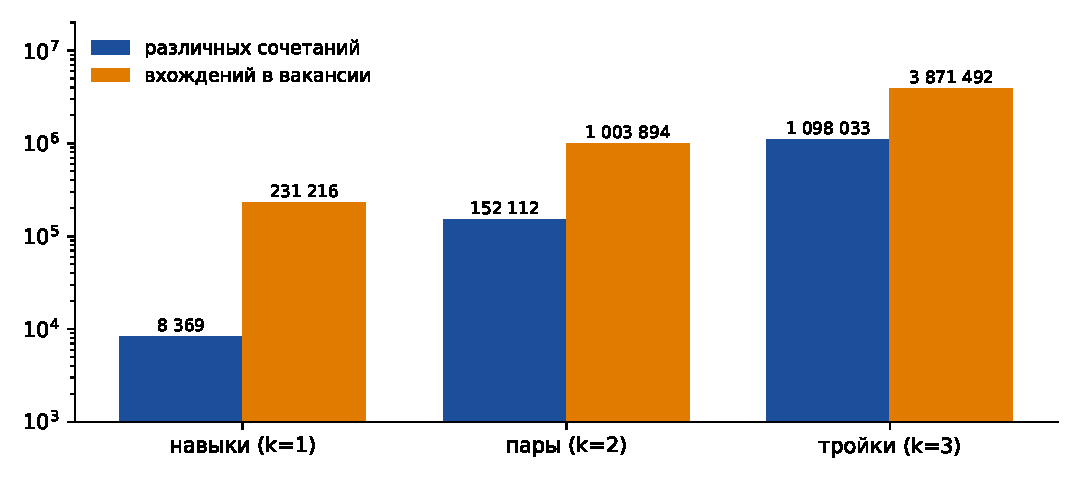
\includegraphics[width=0.78\textwidth]{figures/growth.pdf}
\caption{Различные сочетания и их вхождения в вакансии (логарифмическая шкала).}
\end{figure}

Вакансия с $n$ навыками даёт $\binom{n}{1}=n$ навыков, $\binom{n}{2}$ пар и $\binom{n}{3}$ троек. Сумма по вакансиям в точности равна числу вхождений, которое получил MapReduce:
\[
\sum_i \binom{n_i}{1} = 231\,216, \qquad \sum_i \binom{n_i}{2} = 1\,003\,894, \qquad \sum_i \binom{n_i}{3} = 3\,871\,492 .
\]
В среднем у вакансии $231\,216 / 33\,662 \approx 6{,}9$ навыка, но $\binom{n}{3}$ растёт как $n^3/6$: вакансия-«стажёр» с 29 навыками даёт $\binom{29}{3}=3\,654$ тройки --- больше, чем тысяча вакансий по 3 навыка. Поэтому число вхождений растёт в 4,3 раза от навыков к парам и ещё в 3,9 раза к тройкам, а число \emph{различных} сочетаний --- в 18 и 7 раз: длинный хвост редких навыков порождает миллион почти уникальных троек (1\,098\,033 различных на 3,87~млн вхождений).

\section{Этап 4. Верификация}

\path{verify.py} читает результаты обоих способов из \texttt{hh-lake} и для каждого размера сравнивает \emph{все} строки через \texttt{EXCEPT} в обе стороны, плюс контрольные числа: количество ключей, сумма частот и md5 отсортированного содержимого.

\evidence{04_verify.txt}{Полная сверка MapReduce и DuckDB (verify.py)}

\begin{greenbox}
\textbf{Результат:} для навыков, пар и троек 0 расхождений в обе стороны и одинаковые md5. Во время сверки нашлась только одна проблема --- не в расчёте, а в чтении: автоопределитель формата DuckDB по первым 20\,000 строкам решил, что кавычек в файле троек нет, и споткнулся о навык «закупки, продажи, склад». Формат CSV в \path{verify.py} задан явно.
\end{greenbox}

\subsection{Тест отказа маппера}

\evidence{05_mapper_failure.txt}{Отказ маппера 5 на первой попытке, повтор и повторная сверка}

Мастер перехватил исключение сплита №5, запустил его повторно, итог (26 успешных map-задач, 1 повтор) снова совпал с DuckDB до md5. Повтор безопасен, потому что маппер детерминирован и не имеет побочных эффектов: его результат либо целиком попадает в shuffle, либо отбрасывается.

\section{Профилирование и сравнение подходов (+ бонус)}

\path{profile_runs.py} запускает каждую конфигурацию 3 раза отдельным процессом. Время --- от старта до завершения процесса; пик памяти --- максимум суммарного RSS \emph{всего дерева процессов} (у MapReduce это мастер и воркеры), снимается каждые 50~мс.

\begin{center}
\small
\begin{tabular}{@{}>{\raggedright\arraybackslash}p{5.3cm}>{\raggedright\arraybackslash}p{3.4cm}rp{3.2cm}r@{}}
\rowcolor{accent}\thc{Конфигурация} & \thc{Время, с (3 прогона)} & \thc{Среднее} & \thc{Пик, МБ (3 прогона)} & \thc{Среднее} \\
\tabin{profile}
\bottomrule
\end{tabular}
\end{center}

\begin{figure}[H]
\centering
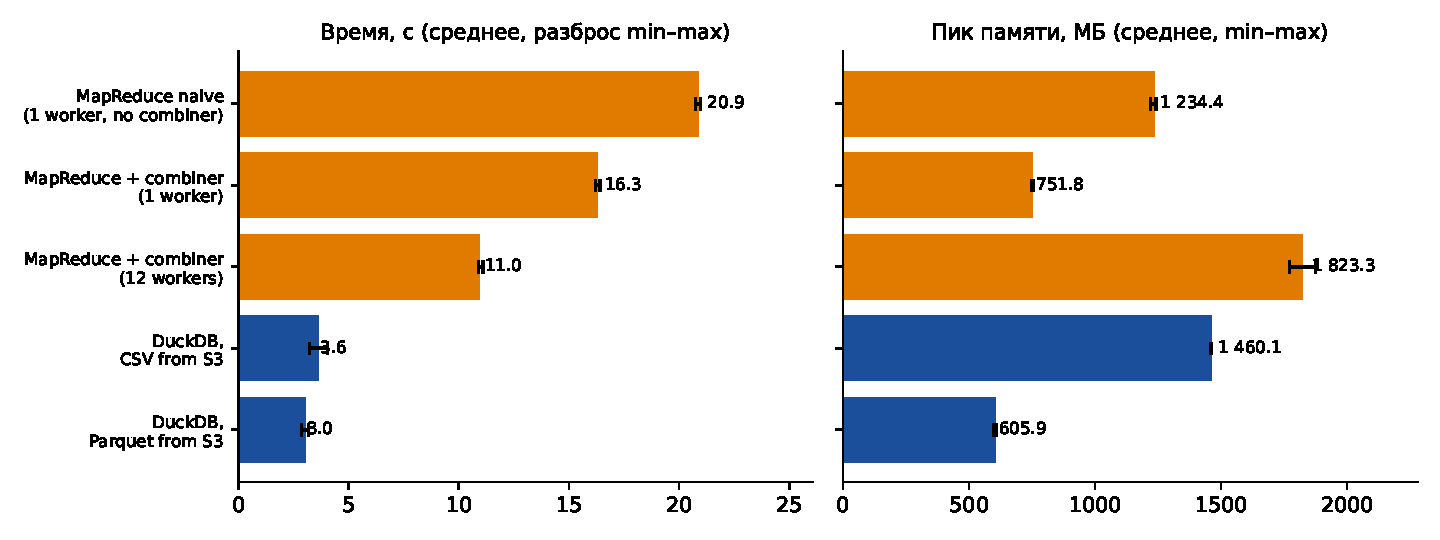
\includegraphics[width=\textwidth]{figures/profile.pdf}
\caption{Время и пик памяти по конфигурациям (оранжевые --- MapReduce, синие --- DuckDB).}
\end{figure}

\evidence{08_profile.txt}{Вывод profile\_runs.py}

\subsection{Что показывают замеры}

\begin{itemize}
\item \textbf{Комбайнер} (наивный MapReduce $\to$ комбайнер, оба в одном воркере): время $20{,}87 \to 16{,}30$~с ($-22\%$), пик памяти $1\,234 \to 752$~МБ ($-39\%$). Без комбайнера маппер отдаёт мастеру каждое вхождение отдельной парой (ключ, 1) --- это $231\,216 + 1\,003\,894 + 3\,871\,492 = 5\,106\,602$ объектов, которые нужно сериализовать, передать между процессами и держать в памяти до свёртки. С комбайнером внутри сплита остаются только различные ключи.
\item \textbf{12 параллельных мапперов}: время $16{,}30 \to 10{,}96$~с, то есть ускорение всего в $1{,}5$ раза, а пик памяти вырос в $2{,}4$ раза ($1\,823$~МБ): 12 интерпретаторов Python, до 24 сплитов по 32~МиБ в работе и частичные счётчики. Ускорение далеко от 12 раз по закону Амдала: последовательными остаются чтение 26 чанков мастером, свёртка в 4 редьюсерах ($\approx1{,}5$~с), формирование и запись в S3 1,1~млн строк троек ($\approx3$~с) и запуск процессов на Windows. Сама map-фаза занимает лишь $\approx3{,}6$~с из 11.
\item \textbf{DuckDB против MapReduce}: $3{,}65$~с против $10{,}96$~с у лучшего MapReduce --- в 3 раза быстрее. Векторный движок на C++ параллельно разбирает CSV и строит хеш-агрегаты, без сериализации данных между процессами Python. Платит памятью ($1\,460$~МБ): параллельный разбор CSV держит в буферах крупные куски файла, а временные таблицы содержат 1,1~млн троек.
\item \textbf{Parquet вместо CSV} для DuckDB: время $3{,}65 \to 3{,}03$~с ($-17\%$), пик памяти $1\,460 \to 606$~МБ ($-58\%$). Parquet колоночный и в 5 раз меньше ($169$ против $848$~МБ): DuckDB читает 3 нужные колонки из 23 и не разбирает самое тяжёлое поле --- текст описания вакансии. Оставшиеся $\approx3$~с --- в основном постоянные затраты (запуск Python, загрузка httpfs, тройное соединение для троек).
\end{itemize}

\evidence{07_make_parquet.txt}{Создание Parquet-копии в hh-lake (make\_parquet.py)}

После профилирования результаты в \texttt{hh-lake} последний раз записали MapReduce на 12 воркерах и DuckDB по \emph{Parquet}; повторная сверка показывает, что и этот путь даёт те же числа:

\evidence{09_verify_after_profile.txt}{Сверка после профилирования: MapReduce (12 воркеров) против DuckDB по Parquet}

\begin{callout}
\textbf{Бонус: «до» и «после».}
\textbf{MapReduce}: $20{,}87$~с / $1\,234$~МБ $\to$ $10{,}96$~с / $1\,823$~МБ (в $1{,}9$ раза быстрее, ценой памяти) или $16{,}30$~с / $752$~МБ (в $1{,}3$ раза быстрее и на 39\% меньше памяти, если ресурс --- память).
\textbf{DuckDB}: $3{,}65$~с / $1\,460$~МБ $\to$ $3{,}03$~с / $606$~МБ (на 17\% быстрее и в $2{,}4$ раза меньше памяти).
Результаты всех вариантов совпадают до md5.
\end{callout}


\section{Этап 5. Как пары и тройки навыков влияют на зарплату}

\subsection{Методика}

\begin{itemize}
\item \textbf{Зарплата:} только RUR; середина вилки или единственная граница; «до вычета налогов» приводится к «на руки» ($\times 0{,}87$); выбросы вне [15~тыс.; 1~млн]~₽ отброшены (их 35, минимум был 43,5~₽). Медиана варианта --- \textbf{93\,960~₽} по 18\,674 вакансиям.
\item \textbf{Прибавка пары} = медиана пары $-$ медиана \emph{более частого} навыка пары (база). \textbf{Прибавка тройки} = медиана тройки $-$ медиана \emph{самой частой} из трёх её пар (база). Так прибавка показывает, что даёт \emph{дополнительный} навык к распространённому стеку.
\item \textbf{Надёжность:} сочетание учитывается, если у него $\ge 30$ вакансий с зарплатой от $\ge 10$ разных работодателей.
\item \textbf{Повторные публикации} одного объявления (тот же работодатель, название, навыки и вилка) считаются одним предложением --- причина ниже. Остаётся 13\,811 предложений с зарплатой (9\,366 с навыками).
\end{itemize}

\begin{warnbox}
\textbf{Найденный артефакт данных.} В первой версии расчёта таблица «понижающих» пар состояла из десятков сочетаний с \texttt{rest} с \emph{одинаковой} медианой 65\,250~₽. Причина: работодатель 6093775 разместил вакансию «Системный аналитик (стажёр)» с вилкой 70--80~тыс. до налогов и списком из 29 навыков в 23 городах; каждая копия давала $\binom{29}{2}=406$ пар и 3\,654 тройки с одной и той же зарплатой. Таких массовых публикаций много:
\end{warnbox}

\begin{center}
\footnotesize
\begin{tabular}{@{}l>{\raggedright\arraybackslash}p{7.2cm}rrrr@{}}
\rowcolor{accent}\thc{Работодатель} & \thc{Вакансия} & \thc{Копий} & \thc{Городов} & \thc{Навыков} & \thc{На руки, ₽} \\
\tabin{mass_postings}
\bottomrule
\end{tabular}
\end{center}

\subsection{Пары, которые сильнее всего повышают и понижают медиану}

{\footnotesize Столбцы: база (более частый навык) и добавленный навык; предложений / работодателей с парой; медиана пары; предложений и медиана базы; прибавка; доля вакансий с опытом 3+ лет у пары / у базы.}

\begin{center}
\footnotesize
\setlength{\tabcolsep}{4pt}
\begin{tabular}{@{}>{\raggedright\arraybackslash}p{2.3cm}>{\raggedright\arraybackslash}p{2.7cm}rrrrlr@{}}
\rowcolor{accent}\thc{База} & \thc{+ навык} & \thc{n / раб.} & \thc{Медиана} & \thc{n базы} & \thc{Мед. базы} & \thc{Прибавка} & \thc{3+ лет} \\
\multicolumn{8}{@{}l}{\cellcolor{okbg}\textbf{Повышают}} \\
\tabin{pairs_up}
\multicolumn{8}{@{}l}{\cellcolor{badbg}\textbf{Понижают}} \\
\tabin{pairs_down}
\bottomrule
\end{tabular}
\end{center}

\subsection{Тройки, которые сильнее всего повышают и понижают медиану}

\begin{center}
\footnotesize
\setlength{\tabcolsep}{4pt}
\begin{tabular}{@{}>{\raggedright\arraybackslash}p{2.9cm}>{\raggedright\arraybackslash}p{2.4cm}rrrrlr@{}}
\rowcolor{accent}\thc{База (частая пара)} & \thc{+ навык} & \thc{n / раб.} & \thc{Медиана} & \thc{n базы} & \thc{Мед. базы} & \thc{Прибавка} & \thc{3+ лет} \\
\multicolumn{8}{@{}l}{\cellcolor{okbg}\textbf{Повышают}} \\
\tabin{triples_up}
\multicolumn{8}{@{}l}{\cellcolor{badbg}\textbf{Понижают}} \\
\tabin{triples_down}
\bottomrule
\end{tabular}
\end{center}

\subsection{Интерпретация}

\textbf{Что повышает зарплату.} Самые сильные прибавки дают навыки интеграционной и архитектурной работы, добавленные к базовому стеку системного аналитика:
\begin{itemize}
\item \textbf{Kafka}: $+139$~тыс. к BPMN, $+133$~тыс. к SQL, $+108$~тыс. к UML; в тройках $+100\ldots105$~тыс. к парам BPMN+UML, BPMN+SQL, SQL+UML. Медиана вакансий с Kafka --- около 300~тыс. на руки.
\item \textbf{Микросервисная архитектура} ($+120{,}5$~тыс. к SQL) и \textbf{системная интеграция} ($+100$~тыс. к SQL), \textbf{XML/JSON} к базам данных и постановке задач ($+90\ldots100$~тыс.).
\item \textbf{A/B-тесты} к Python ($+105$~тыс.) и к паре Python+SQL ($+100$~тыс.) --- продуктовая аналитика с экспериментами.
\item \textbf{ERP-системы на базе 1С} и \textbf{бухгалтерский учёт} к «сбору и анализу информации» ($+120$~тыс.): узкая и дорогая ниша внедрения ERP.
\end{itemize}

\textbf{Что понижает.} Сильнее всего медиану тянут вниз \emph{общие} формулировки, добавленные к технической базе: «работа с базами данных» к REST ($-120$~тыс.), «аналитический склад ума» к системному анализу ($-95$~тыс.), «оптимизация бизнес-процессов» к UML ($-89$~тыс.), MS Excel, анализ рынка, аналитические исследования ($-69\ldots80$~тыс.). В тройках --- «информационные технологии», «аналитическое мышление», «техническая документация» к дорогим парам с REST/SOAP ($-90\ldots106$~тыс.). Неожиданно понижает и \textbf{Python} в тройке с BPMN+SQL ($-95$~тыс.): такой набор характерен не для системных аналитиков, а для начинающих аналитиков данных и бизнес-аналитиков.

\begin{callout}
\textbf{Главное объяснение --- опыт, а не навык сам по себе.} В последнем столбце таблиц видно: у повышающих пар доля вакансий с опытом от 3 лет 43--97\% (у большинства выше 55\%) против 21--52\% у базы, а у понижающих --- 3--50\% при 34--62\% у базы. Технические интеграционные навыки работодатели перечисляют в вакансиях для опытных системных аналитиков, а общие и «мягкие» формулировки --- в вакансиях для начинающих и в массовых объявлениях (например, стажёрские вакансии работодателя 6093775 с медианой 65\,250~₽). Поэтому прибавка --- это описание рынка, а не обещание: выучив Kafka без опыта, зарплату в 300~тыс. не получить.
\end{callout}


\section{Этап 6. Региональный анализ: Москва, Санкт-Петербург, Екатеринбург}

Выбраны три крупнейших рынка варианта (26\,726, 5\,793 и 2\,203 вакансии). Регионы сравниваются по всем вакансиям региона (здесь копии вакансии в разных городах законно относятся к разным регионам).

\subsection{Ключевые показатели}

\begin{center}
\footnotesize
\setlength{\tabcolsep}{3.5pt}
\begin{tabular}{@{}lrrrrrrrrrr@{}}
\rowcolor{accent}\thc{Регион} & \thc{Вакансий} & \thc{С навык.} & \thc{Навыков} & \thc{С з/п} & \thc{P25} & \thc{Медиана} & \thc{P75} & \thc{Удалёнка} & \thc{Без опыта} & \thc{3+ лет} \\
\tabin{regions_metrics}
\bottomrule
\end{tabular}
\end{center}

\begin{figure}[H]
\centering
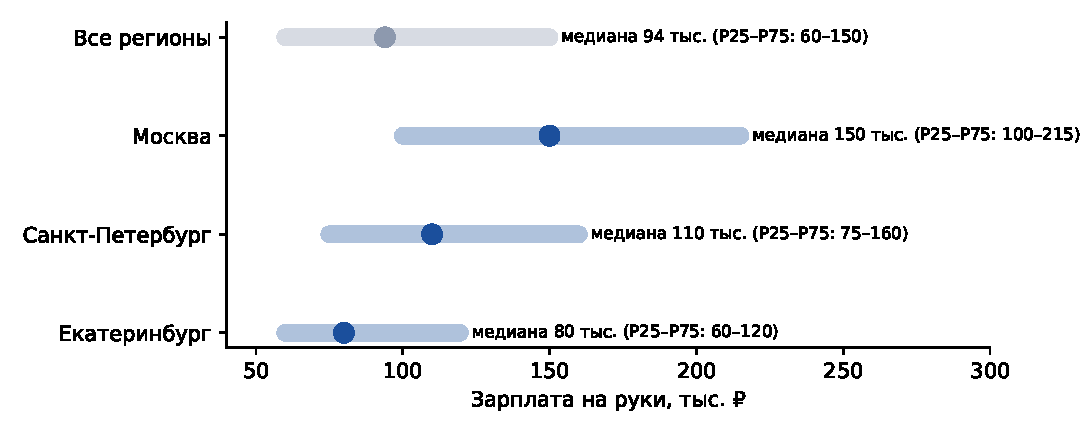
\includegraphics[width=0.85\textwidth]{figures/regions.pdf}
\caption{Медиана и межквартильный размах зарплаты по регионам.}
\end{figure}

\subsection{Самые востребованные навыки, пары и тройки}

{\footnotesize В ячейке: сочетание; число вакансий, доля от вакансий региона с навыками, медиана зарплаты.}

\begin{center}
\scriptsize
\setlength{\tabcolsep}{3pt}
\begin{tabular}{@{}l>{\raggedright\arraybackslash}p{5.3cm}>{\raggedright\arraybackslash}p{5.3cm}>{\raggedright\arraybackslash}p{5.3cm}@{}}
\rowcolor{accent}\thc{\#} & \thc{Москва} & \thc{Санкт-Петербург} & \thc{Екатеринбург} \\
\multicolumn{4}{@{}l}{\cellcolor{infobg}\textbf{Навыки}} \\
\tabin{regions_top_k1}
\multicolumn{4}{@{}l}{\cellcolor{infobg}\textbf{Пары}} \\
\tabin{regions_top_k2}
\multicolumn{4}{@{}l}{\cellcolor{infobg}\textbf{Тройки}} \\
\tabin{regions_top_k3}
\bottomrule
\end{tabular}
\end{center}

\subsection{Характерные навыки регионов и цена одинаковых навыков}

\begin{center}
\footnotesize
\begin{tabular}{@{}llrrrr@{}}
\rowcolor{accent}\thc{Регион} & \thc{Навык} & \thc{Вакансий} & \thc{Доля} & \thc{В двух других} & \thc{Отношение} \\
\tabin{regions_distinctive}
\bottomrule
\end{tabular}
\end{center}

\begin{center}
\footnotesize
\begin{tabular}{@{}lrrr@{}}
\rowcolor{accent}\thc{Навык (8 самых частых)} & \thc{Москва} & \thc{Санкт-Петербург} & \thc{Екатеринбург} \\
\tabin{regions_skill_salary}
\bottomrule
\end{tabular}

{\footnotesize Медиана зарплаты на руки, ₽; в скобках --- число вакансий с зарплатой.}
\end{center}

\subsection{Наблюдения}

\begin{itemize}
\item \textbf{Москва --- половина рынка и самые высокие зарплаты.} 26\,726 из 54\,607 вакансий варианта (49\%). Медиана 150~тыс. на руки --- на 36\% выше Петербурга (110~тыс.) и на 88\% выше Екатеринбурга (80~тыс.). Даже нижний квартиль Москвы (100~тыс.) выше медианы Екатеринбурга.
\item \textbf{Разрыв объясняется и составом вакансий, и ценой навыка.} В Москве больше вакансий для опытных: 46\% с опытом от 3 лет против 38\% в Петербурге и 26\% в Екатеринбурге; без опыта --- 6\%, 9\% и 11\%. Но и за \emph{одинаковый} навык Москва платит больше: SQL --- 174 / 125 / 104~тыс., системный анализ --- 200 / 150 / 120~тыс., UML --- 218 / 150 / 138~тыс. Надбавка Москвы за тот же навык --- от трети до двух третей.
\item \textbf{Удалёнка не выравнивает рынок.} Доля удалённых вакансий почти одинакова (24--25\% во всех трёх регионах), но зарплаты по-прежнему привязаны к городу публикации.
\item \textbf{Разный спрос на навыки.} В Москве и Петербурге первый навык --- SQL (37,6\% и 30,5\% вакансий с навыками), в Екатеринбурге --- «аналитическое мышление» (29,4\%), SQL только второй. Тройка BPMN + SQL + UML --- самая частая во всех трёх регионах, то есть ядро системного аналитика общее; различаются окраины.
\item \textbf{Характерные навыки показывают профиль рынка.} Москва --- большие данные и хранилища: Hadoop (в 3,3 раза чаще, чем в двух других регионах), Greenplum (3,1×), DWH (2,1×) --- банки и крупные IT-компании. Петербург --- внедрение 1С ERP: 1С:УП, 1С:КА, 1С:ERP, 1С:УПП (2,2--2,5×) --- производственные и торговые компании. Екатеринбург --- общие формулировки («аналитический склад ума», «работа в команде», «информационные технологии») и программирование 1С: вакансии менее специализированы, что согласуется с самой низкой медианой.
\item \textbf{Чем не различаются.} Доля вакансий с навыками (60--65\%) и длина списка навыков (6,7--6,8) почти одинаковы: регионы различаются не количеством требований, а их содержанием и ценой.
\end{itemize}


\section{Ограничения и допущения}

\begin{itemize}
\item Вариант определён по полю \texttt{role}; аналитики с другой ролью (например, «Программист» в названии которого есть «аналитик») не входят.
\item Зарплата приводится к «на руки» единым коэффициентом 0,87; прогрессивная шкала НДФЛ не учитывается. Вакансии в других валютах (около 1\%) исключены.
\item Медианы зарплат --- описательная статистика, а не причинный эффект: навык коррелирует с опытом, городом и работодателем (это видно по столбцу «3+ лет»).
\item Хранилище --- учебный кластер на одном физическом диске (см. ДЗ №2); время чтения из S3 здесь почти равно времени чтения с локального диска.
\item Замеры --- 3 прогона на одной машине (12 логических ядер, 34~ГБ RAM); пик памяти снимается с шагом 50~мс и может недооценивать кратковременные всплески.
\end{itemize}

\section{Воспроизведение}

Код и отчёт: \IfFileExists{repo_url.tex}{\url{https://github.com/nalivo4ka/DataEngeneering-hw3-mapreduce-rustfs}
}{репозиторий GitHub (ссылка в README)}. Порядок запуска: \path{upload_raw.py} $\to$ \path{mapreduce.py} $\to$ \path{duckdb_counts.py} $\to$ \path{verify.py} $\to$ \path{mapreduce.py --fail-map-task 5} $\to$ \path{analysis.py} $\to$ \path{make_parquet.py} $\to$ \path{profile_runs.py} $\to$ \path{make_figures.py}, \path{make_tables.py}. Все выводы запусков лежат в \path{logs/}, таблицы анализа --- в \path{out/} и \path{s3://hh-lake/results/analysis/}.

\end{document}
